%%%%%%%%%%%%%%%%%%%%%%%%%%%%%%%%%%%%%%%%%
% Beamer Presentation
% LaTeX Template
% Version 1.0 (10/11/12)
%
% This template has been downloaded from:
% http://www.LaTeXTemplates.com
%
% License:
% CC BY-NC-SA 3.0 (http://creativecommons.org/licenses/by-nc-sa/3.0/)
%
%%%%%%%%%%%%%%%%%%%%%%%%%%%%%%%%%%%%%%%%%

%----------------------------------------------------------------------------------------
%	PACKAGES AND THEMES
%----------------------------------------------------------------------------------------

\documentclass{beamer}

\mode<presentation> {

% The Beamer class comes with a number of default slide themes
% which change the colors and layouts of slides. Below this is a list
% of all the themes, uncomment each in turn to see what they look like.

%\usetheme{default}
%\usetheme{AnnArbor}
%\usetheme{Antibes}
%\usetheme{Bergen}
%\usetheme{Berkeley}
%\usetheme{Berlin}
%\usetheme{Boadilla}
%\usetheme{CambridgeUS}
%\usetheme{Copenhagen}
%\usetheme{Darmstadt}
%\usetheme{Dresden}

%\usetheme{Frankfurt}

%\usetheme{Goettingen}
%\usetheme{Hannover}
\usetheme{Ilmenau}
%\usetheme{JuanLesPins}
%\usetheme{Luebeck}

%\usetheme{Madrid}

%\usetheme{Malmoe}
%\usetheme{Marburg}
%\usetheme{Montpellier}
%\usetheme{PaloAlto}
%\usetheme{Pittsburgh}

%\usetheme{Rochester}
%\usetheme{Singapore}

%\usetheme{Szeged}
%\usetheme{Warsaw}

% As well as themes, the Beamer class has a number of color themes
% for any slide theme. Uncomment each of these in turn to see how it
% changes the colors of your current slide theme.

%\usecolortheme{albatross}
%\usecolortheme{beaver}
%\usecolortheme{beetle}
%\usecolortheme{crane}
%\usecolortheme{dolphin}
%\usecolortheme{dove}
%\usecolortheme{fly}
%\usecolortheme{lily}
%\usecolortheme{orchid}
%\usecolortheme{rose}
%\usecolortheme{seagull}
%\usecolortheme{seahorse}
%\usecolortheme{whale}
%\usecolortheme{wolverine}

%\setbeamertemplate{footline} % To remove the footer line in all slides uncomment this line
%\setbeamertemplate{footline}[page number] % To replace the footer line in all slides with a simple slide count uncomment this line

%\setbeamertemplate{navigation symbols}{} % To remove the navigation symbols from the bottom of all slides uncomment this line
}

\usepackage{graphicx} % Allows including images
\usepackage{booktabs} % Allows the use of \toprule, \midrule and \bottomrule in tables
\usepackage{array}
\usepackage{color}
\usepackage{url}
\usepackage[T2A]{fontenc}
\usepackage[utf8]{inputenc}
\usepackage[export]{adjustbox}
\usepackage{amsmath}
\usepackage{sidecap}
\usepackage{listings}
\usepackage{mathtools}
\usepackage[normalem]{ulem}
\usepackage[english,serbian]{babel}
%\usepackage[english,serbianc]{babel} %ukljuciti babel sa ovim opcijama, umesto gornjim, ukoliko se koristi cirilica

\lstset{breakatwhitespace,
language=C++,
columns=fullflexible,
keepspaces,
breaklines,
tabsize=4,
showstringspaces=false,
basicstyle=\ttfamily,
extendedchars=true}

\AtBeginSection[]
{
    \begin{frame}<beamer>
        \frametitle{Sadržaj}
        \tableofcontents[currentsection]
    \end{frame}

}


%----------------------------------------------------------------------------------------
%	TITLE PAGE
%----------------------------------------------------------------------------------------

\title[]{Klasifikacija muzejskih slika korišćenjem dubokih konvolutivnih neuronskih mreža}
\author{Nemanja Mićović \\ \texttt{nemanja\_micovic@matf.bg.ac.rs} \\ \texttt{machinelearning.matf.bg.ac.rs}}
\institute[MATF]{Matematički fakultet \\ Univerzitet u Beogradu}
\date{\today}

\begin{document}

\begin{frame}
    \titlepage
\end{frame}

\begin{frame}
\frametitle{Sadržaj}
\tableofcontents
\end{frame}

%----------------------------------------------------------------------------------------
%	PREZENTACIJA
%----------------------------------------------------------------------------------------
%-----------------------------------------------------------------
\section{Uvod}
%\begin{frame}
    %\frametitle{Машинско учење}
    %\framesubtitle{Стабло одлучивања}
    %\begin{figure}
        %\centering
        %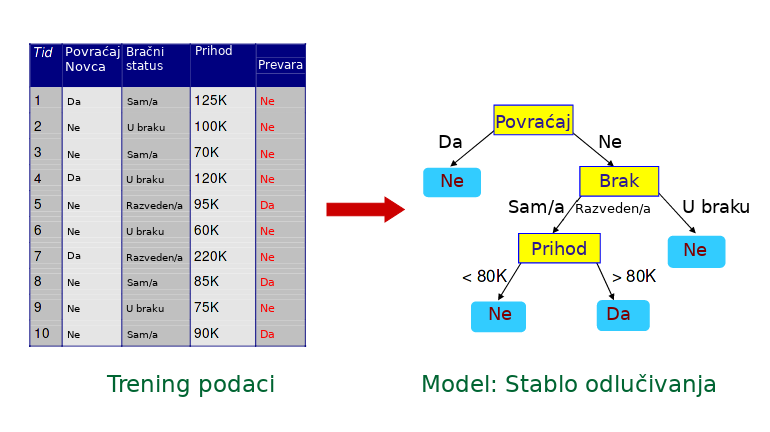
\includegraphics[scale=0.4]{slike/decision_tree.png}
    %\end{figure}
%\end{frame}
%-----------------------------------------------------------------
\begin{frame}{Neki od važnijih rezultata mašinskog učenja}
    \begin{itemize}
        \item 1992 - TD-Gammon, sistem koji igra igru Tavla, razvijen od strane Džeralda Tezaura
        \item 2011 - IBM-om Watson pobeđuje u kvizu \textit{Jeopardy!}
        \item 2012 - Google X sistem koji prepoznaje mačke na video snimcima
        \item 2015 - Greška klasifikacije slika na ILSVRC 2015 od 3.6\%
        \item 2016 - Sistem AlphaGo pobeđuje svetskog šampiona sa 4:1
        \item 2017 - AlphaGo igra protiv sebe iz 2016. godine i 100 partija pobeđuje 100
    \end{itemize}
\end{frame}
%-----------------------------------------------------------------
\begin{frame}{Neke od primena mašinskog učenja}
    \begin{itemize}
        \item Autonomna vožnja
        \item Algoritamski portfolio
        \item Igranje video igara
        \item Generisanje algoritama optimizacije \cite{learning-to-learn}
        \item Klasifikacija slika
        \item Prepoznavanje rukopisa
        \item Generisanje slika
        \item Obrada prirodnih jezika
        \item Bioinformatika
        \item Društvene mreže
    \end{itemize} 
\end{frame}
%-----------------------------------------------------------------
\begin{frame}{Neuronske mreže}
    \begin{itemize}
        \item Univerzalni aproksimatori funkcija 
        \item U osnovi mnogih popularnih algoritama mašinskog učenja
        \item Više o njima u \cite{Murphy, Bishop, Goodfellow}
    \end{itemize}

    \begin{center}
        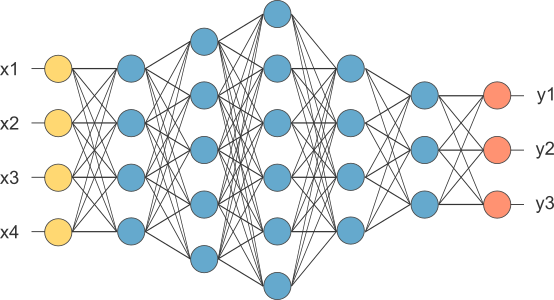
\includegraphics[scale=0.5]{./slike/deep_neural_network.png}
    \end{center}
\end{frame}
%-----------------------------------------------------------------
\begin{frame}{Neuron neuronske mreže}
    \begin{columns}
    \begin{column}{0.5\textwidth}
        Terminologija:
        \begin{itemize}
            \item Ulaz neurona: $a_i$
            \item Težine neurona: $w_i$
            \item Slobodni član: $b$
            \item Nelinearna funkcija: $g$
        \end{itemize}

        Izlaz neurona se izračunava po formuli:
        $$
            a_{out} = g(b + \sum_{i=1}^{N} a_i w_i)
        $$
    \end{column}
    \begin{column}{0.5\textwidth}  %%<--- here
        \begin{center}
            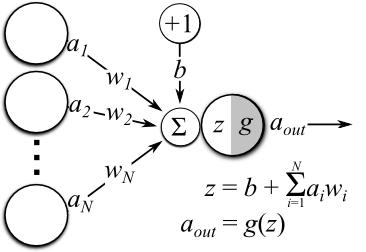
\includegraphics[scale=0.9]{./slike/neuron.png}
        \end{center}
    \end{column}
    \end{columns}
\end{frame}
%-----------------------------------------------------------------
\begin{frame}{Aktivacione funkcije neuronske mreže}
    \begin{itemize}
        \item Vrlo je bitno primeniti nelinearnu transformaciju inače će funkcija ostati linearna
        \item Neke od popularnih aktivacionih funkcija:
        \begin{itemize}
            \item ReLU: $ g(x) = max(0, x)$
            \item Sigmoidna funkcija: $ g(x) = \frac{1}{1 + e^{-x}} $
            %\item Tangens hiperbolički$ g(x) = \frac{1 - e^{-2x}}{1 + e^{-2x}} $
            \item Tangens hiperbolički $ g(x) = \frac{e^x - e^{-x}}{e^x + e^{-x}} $
        \end{itemize}
    \end{itemize}
\end{frame}
%-----------------------------------------------------------------
\begin{frame}{Trening neuronskih mreža}
    Propagacija unazad (eng. backpropagation)
    \begin{itemize}
        \item Izračunava gradijent funkcije greške u odnosu na težine neurona
        \item Predstavlja osnovu algoritama za trening neuronskih mreža
    \end{itemize}

    Grafičke karte omogućavaju da se efikasno paralelizuju mnoge od potrebnih operacija
    za trening neuronskih mreža.
\end{frame}
%-----------------------------------------------------------------
\begin{frame}{Konvolutivne mreže}
    \begin{itemize}
        \item Vrsta neuronskih mreža
        \item Prilagođena obradi signala u kojima postoji prostorna lociranost (slika, zvuk, video)
        \item Mogu vršiti konstrukciju relevantnih atributa
        \item Kompleksnost atributa koji se prepoznaje raste sa dubinom mreže
    \end{itemize}
\end{frame}
%-----------------------------------------------------------------
\begin{frame}{Konvolutivne mreže}
    \begin{center}
        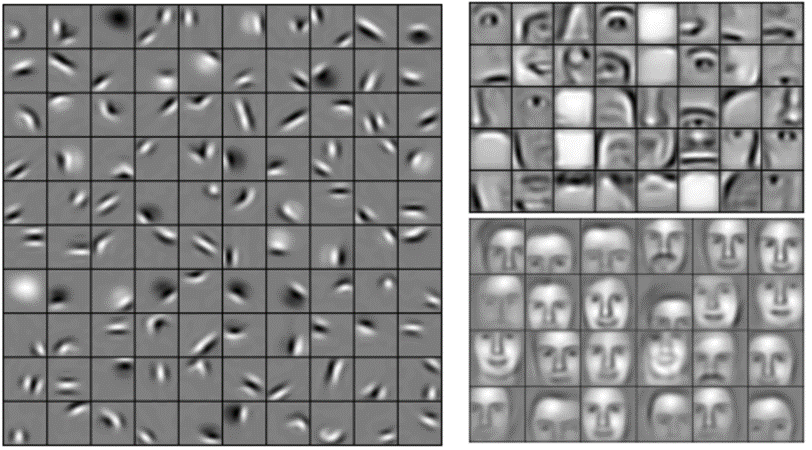
\includegraphics[width=\textwidth]{./slike/covnet-visual01.png}
    \end{center}
\end{frame}
%-----------------------------------------------------------------
\begin{frame}{Konvolutivne mreže}
    \begin{center}
        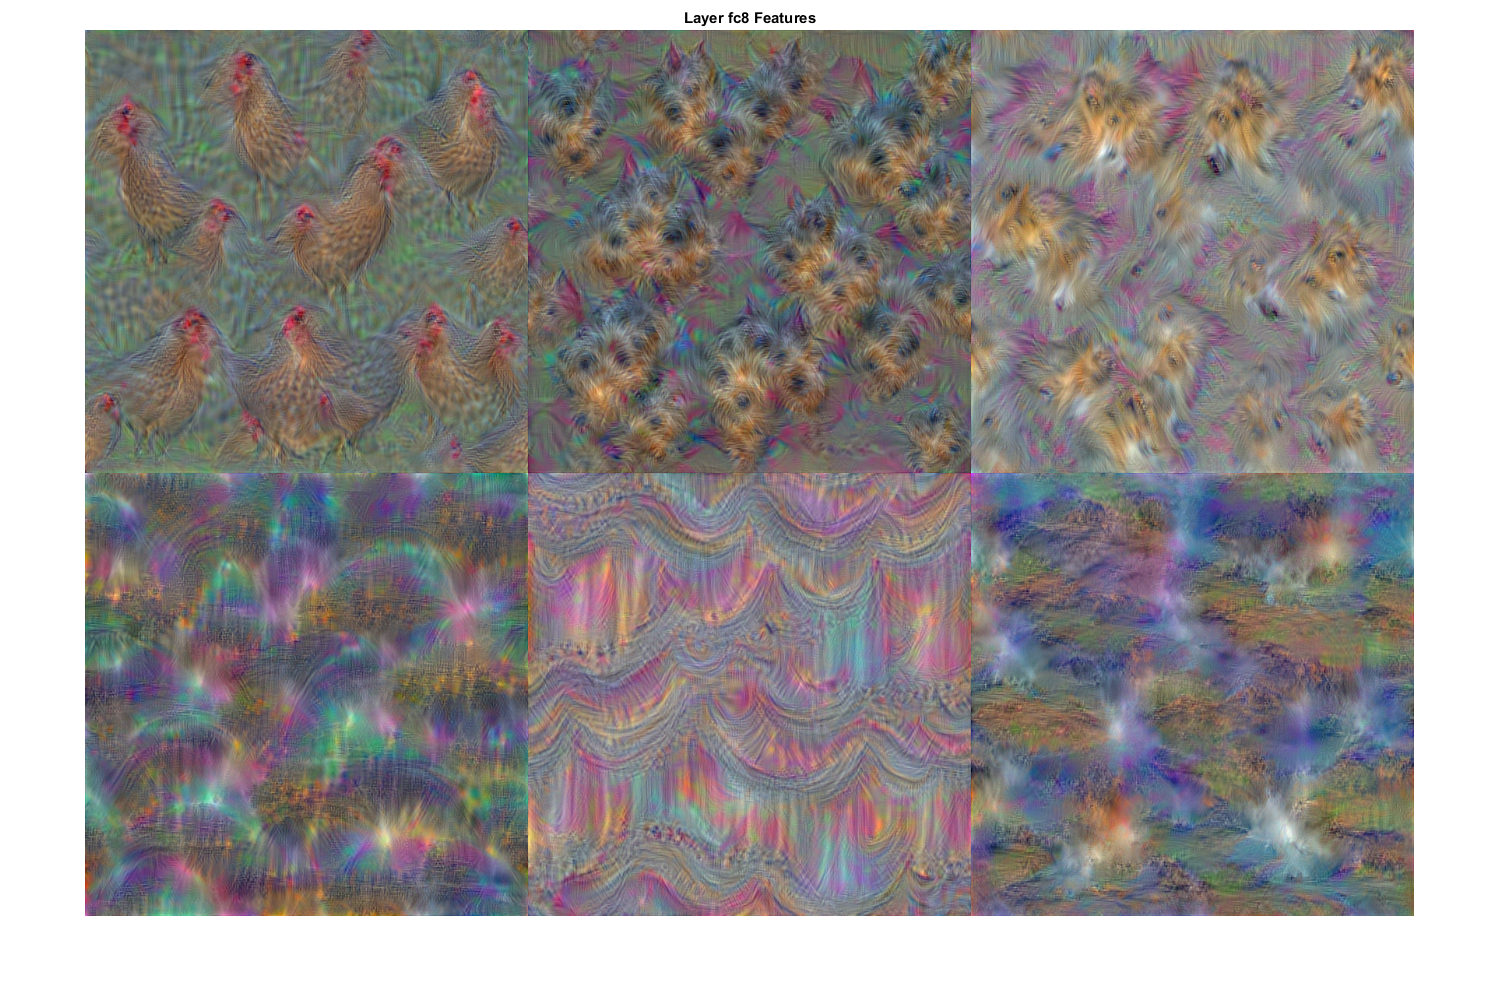
\includegraphics[width=\textwidth]{./slike/covnet-visual02.png}
    \end{center}
\end{frame}
%-----------------------------------------------------------------
\begin{frame}{Konvolutivne mreže - arhitektura}
    Arhitektura se sastoji iz kombinacije sledećih elemenata:
    \begin{itemize}
        \item Sloj konvolucije
        \item Sloj agregacije
        \item Standardna neuronska mreža
    \end{itemize}
\end{frame}
%-----------------------------------------------------------------
\begin{frame}{Konvolutivne mreže - arhitektura}
    Konvolutivni sloj:
    \begin{itemize}
        \item Služi da detektuje određenu pravilnost u podacima
        \item Na primer, da detektuje horizontalne, vertikalne i kose linije (niži sloj) ili oči, uši i usne (viši sloj)
    \end{itemize}
\end{frame}
%-----------------------------------------------------------------
\begin{frame}{Konvolutivne mreže - arhitektura}
    Agregatni sloj (eng. pooling):
    \begin{itemize}
        \item Ukrupnjava informaciju iz prethodnog sloja (uglavnom je to konvolutivni sloj)
        \item Kao funkcija ukrupnjavanja se koristi maksimum ili prosek
    \end{itemize}

    \begin{center}
        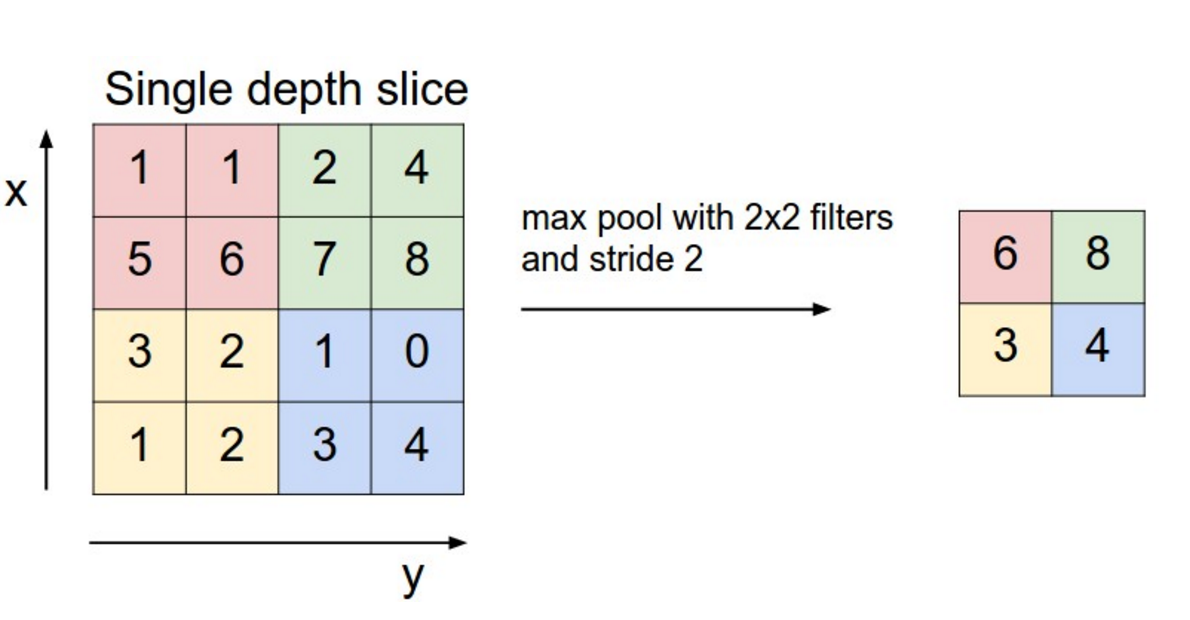
\includegraphics[width=\textwidth]{./slike/maxpooling.png}
    \end{center}
\end{frame}
%-----------------------------------------------------------------
\begin{frame}{Konvolutivne mreže - arhitektura}
    Standardna neuronska mreža:
    \begin{itemize}
        \item Vrši klasifikaciju nad atributima koji su konstruisani u prethodnim slojevima
    \end{itemize}
\end{frame}
%-----------------------------------------------------------------
\begin{frame}{Konvolutivne mreže - arhitektura}
    \begin{center}
        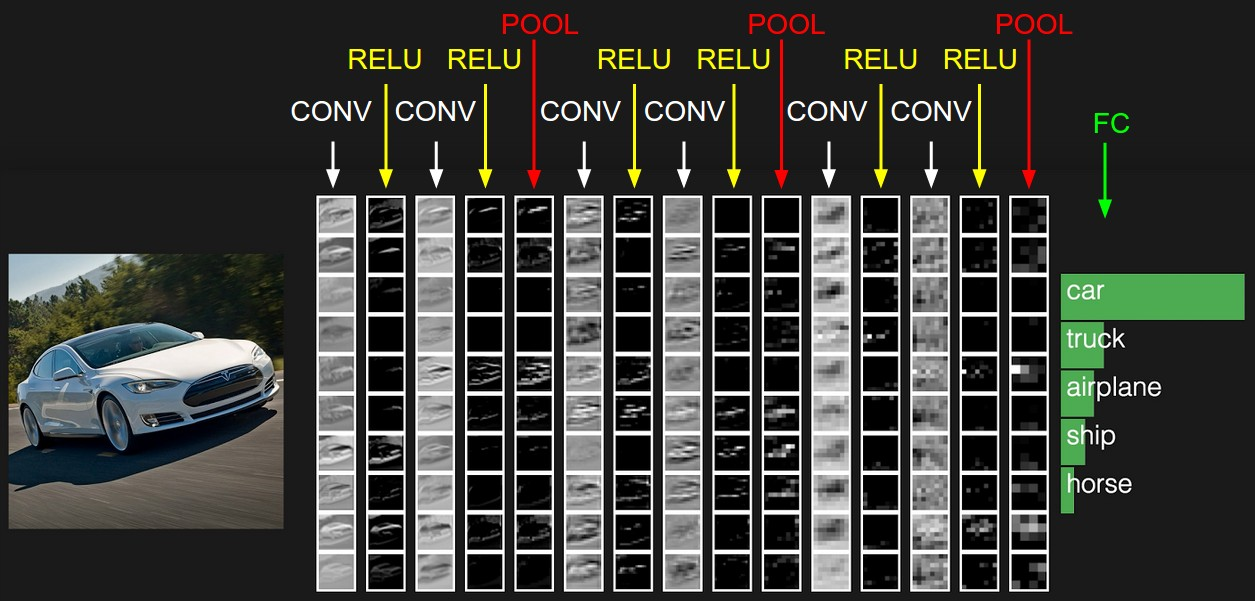
\includegraphics[width=\textwidth]{./slike/convnet01.jpeg}
    \end{center}
\end{frame}
%-----------------------------------------------------------------

%-----------------------------------------------------------------
\section{Problem klasifikacije muzejskih slika}
%-----------------------------------------------------------------
\begin{frame}{Zahtevi}
    Želimo da korisnicima omogućimo da:
    \begin{itemize}[<+->]
        \item fotografišu sliku na zidu i dobiju odgovor šta/ko je na njoj
        \item ne čekaju duže od 5 sekundi na odgovor
        \item kvalitet fotografije ne utiče drastično na preciznost klasifikacije
        \item da rezolucija fotografije ne utiče na preciznost klasifikacije
        \item da ugao slike minimalno utiče na preciznost klasifikacije
        \item da klasifikator skoro nikada ne greši
        \item to sve radi na mobilnim uređajima (i njihovim različitim platformama)
        \item mobilni uređaj ne pregori dok se vrši klasifikacija.
    \end{itemize}
\end{frame}
%-----------------------------------------------------------------
\begin{frame}{Alati za klasifikaciju slika}
    \begin{itemize}
        \item Izabrana je konvolutivna mreža usled zahteva o preciznosti i robusnosti klasifikatora
        \item Konvolutivne mreže imaju višegodišnji uspeh u klasifikaciji slika \cite{krizhevsky, microsoftCovnet, r-cnn, cnn-rnn-semantic}
        \item Time je teže ispuniti ograničenje o podržanim platformama i problemu rada na mobilnom uređaju 
    \end{itemize}
\end{frame}
%-----------------------------------------------------------------
\section{Arhitektura aplikacije}
%-----------------------------------------------------------------
\begin{frame}{Rešavanje problema podržavanja platformi - rešenje 1}
    Iako postoje biblioteke koje rade na sistemima Android i iOS:
    \begin{itemize}
        \item zahtevaju pisanje odvojenih kodova (duplira se posao)
        \item nisu dovoljno popularne i korišćene, teško je dobiti podršku ukoliko se javi neki problem
        \item mobilni uređaji potencijalno nisu dovoljno hardverski snažni
        \item ažuriranje modela klasifikacije nije trivijalno (treba svaki korisnik da ažurira aplikaciju)
        \item kako proširiti skup podataka od korisničkih fotografija?
    \end{itemize}
\end{frame}
%-----------------------------------------------------------------
\begin{frame}{Rešavanje problema podržavanja platformi - rešenje 2}
    Potencijalno rešenje:
    \begin{itemize}
        \item Dobijeni klasifikator (treningom konvolutivne mreže) postavljamo na javno dostupan server
        \item Mobilne aplikacije koriste uslugu servera (server pruža REST \cite{rest} API\footnote{Application programming interface})
        \begin{itemize}
            \item Za poslatu sliku, dobijaju klasu kojoj slika pripada
        \end{itemize}
    \end{itemize}
\end{frame}
%-----------------------------------------------------------------
\begin{frame}{Dobre strane}
    \begin{itemize}
        \item Ne opterećuje se više mobilni uređaj
        \item Za klasifikator možemo koristiti proizvoljnu biblioteku za mašinsko učenje
        \item Model se može trenirati bilo gde
        \item Na serveru možemo čuvati nove korisničke fotografije i proširiti skup podataka
        \item Ažuriranje klasifikatora istovremeno ažurira svim korisnicma preciznost na mobilnim uređajima
    \end{itemize}
    \begin{center}
        
\includegraphics[scale=0.18]{./slike/thumbs_up.png}
    \end{center}
\end{frame}
%-----------------------------------------------------------------
\begin{frame}{Loše strane}
    \begin{itemize}
        \item Neophodna je internet konekcija
        \item Velika količina istovremenih zahteva može stvoriti problem pri klasifikaciji
        \item Potreban server koji omogućava korišćenje biblioteka za mašinsko učenje
        \item Potencijalni bezbednosni propusti
        \item Održavanje servera
    \end{itemize}
    \begin{center}
        
\includegraphics[scale=0.23]{./slike/thumbs_down.png}
    \end{center}
\end{frame}
%-----------------------------------------------------------------
\begin{frame}{Arhitektura}
    % TODO: dodati sliku
    \begin{center}
        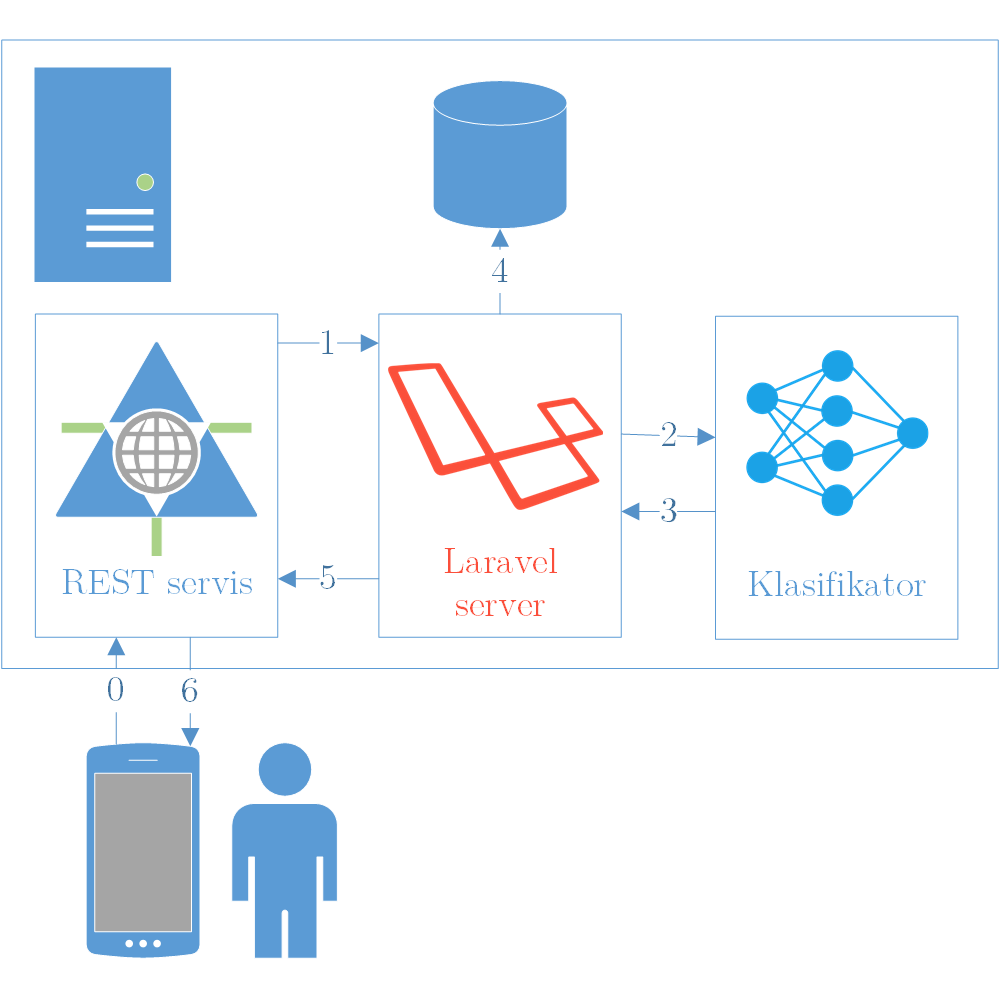
\includegraphics[scale=0.3]{./slike/arch.png}
    \end{center}
\end{frame}
%-----------------------------------------------------------------
\begin{frame}{Primer}
\begin{columns}
\begin{column}{0.5\textwidth}
    \begin{center}
        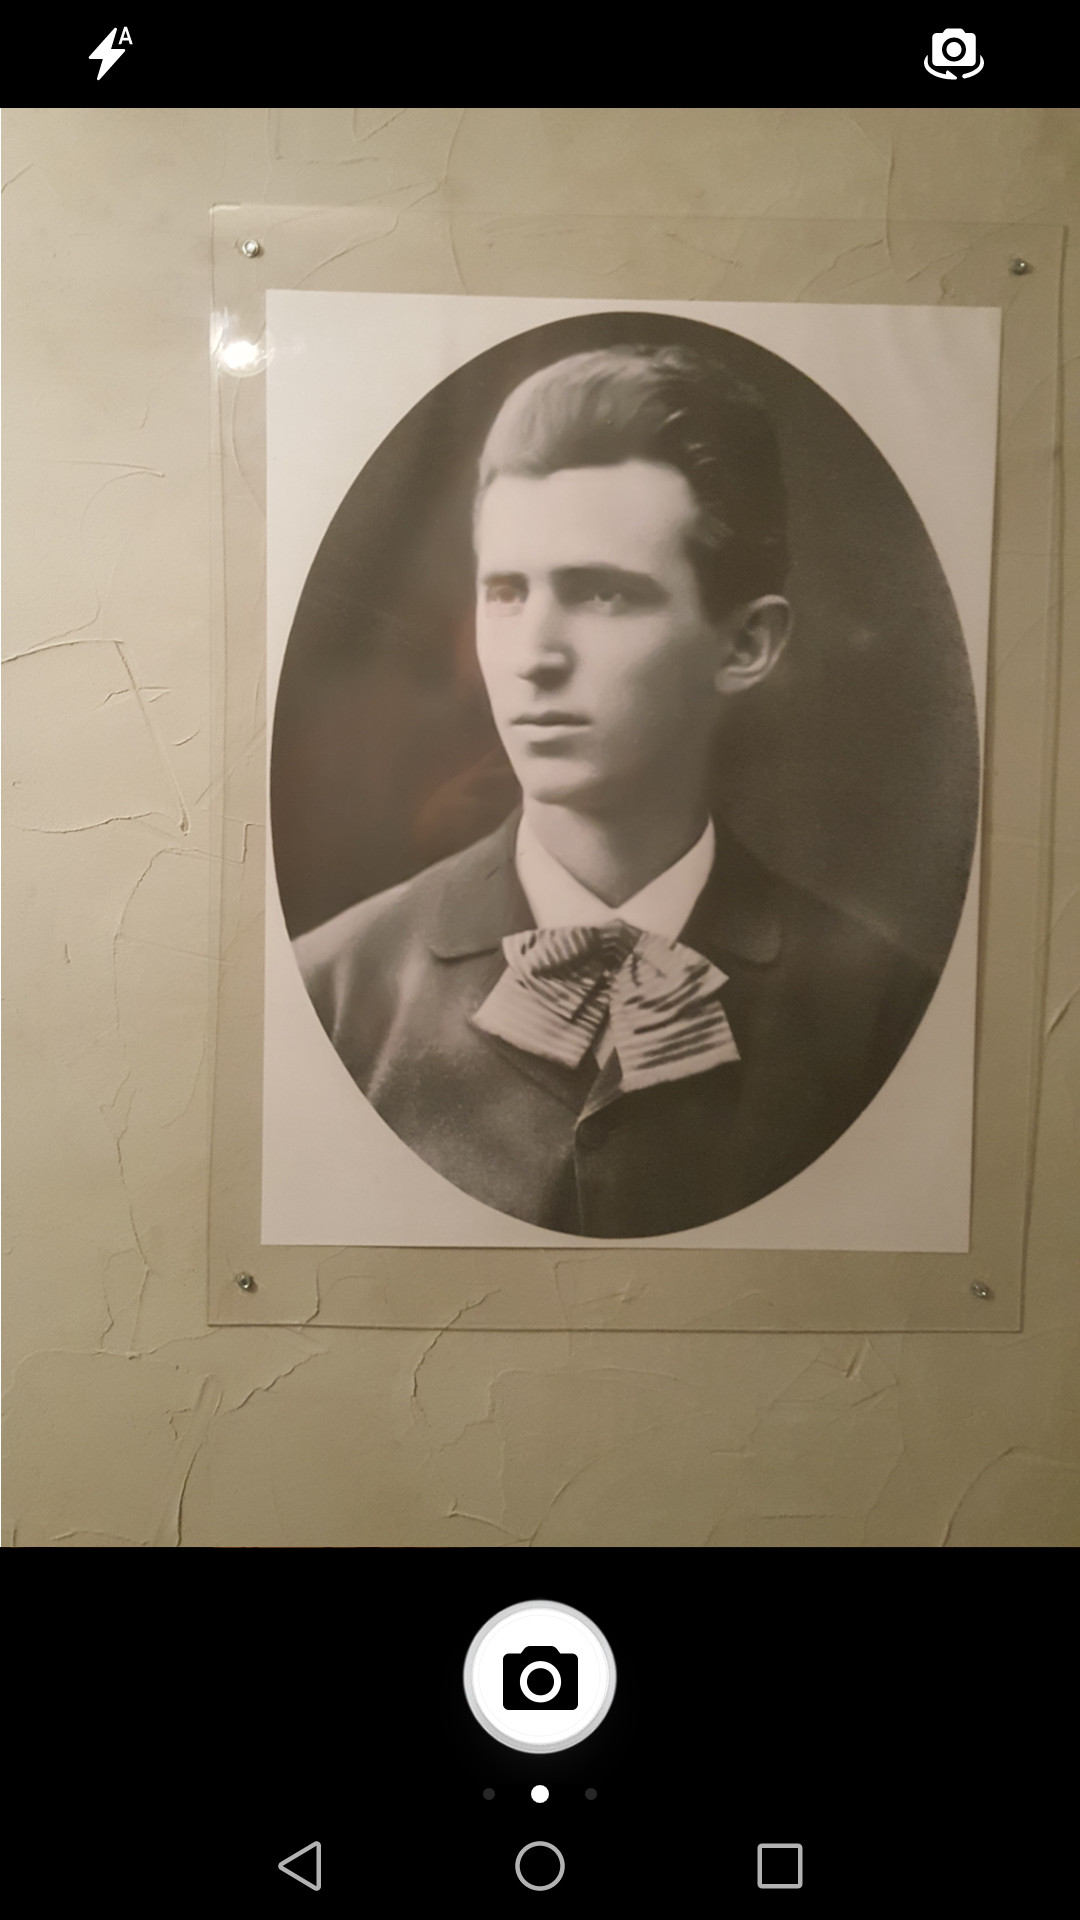
\includegraphics[scale=0.093]{./slike/young_tesla_real.jpg}
    \end{center}
\end{column}
\begin{column}{0.5\textwidth}
    \begin{center}
        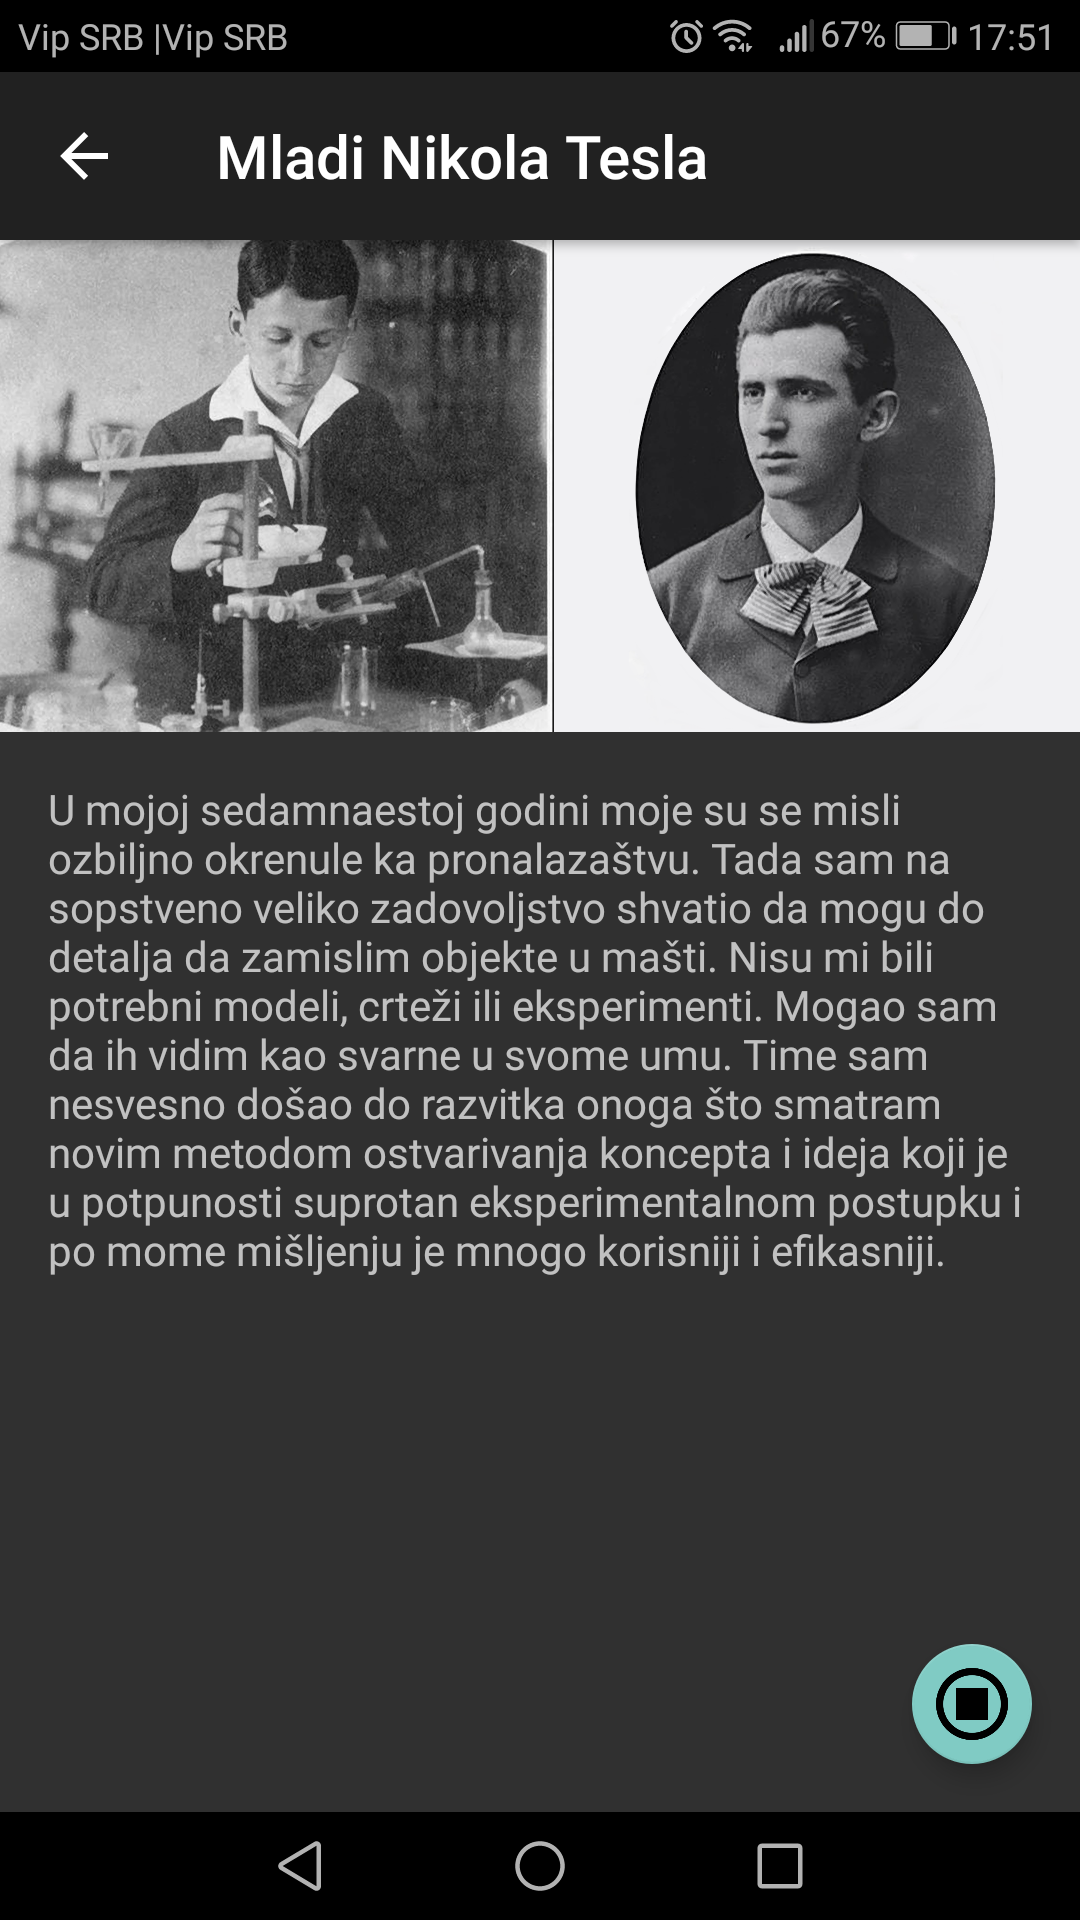
\includegraphics[scale=0.093]{./slike/young_tesla_app.png}
    \end{center}
\end{column}
\end{columns}
\end{frame}

%-----------------------------------------------------------------
\section{Preprocesiranje i trening}
%-----------------------------------------------------------------
\begin{frame}{Skup podataka}
    \begin{itemize}
        \item Potrebno napraviti skup podataka
        \item U muzeju postoji 9 slika na zidu (dakle 9 klasa)
        \item Za početak napravljen skup podataka od 1800 slika (200 slika po klasi)
        \begin{itemize}
            \item Trening konvolutivne mreže prošao (očekivano) katastrofalno
            \item Preciznost oko 0.3
        \end{itemize}
    \end{itemize} 
\end{frame}
%-----------------------------------------------------------------
\begin{frame}{Proširivanje skupa podataka}
    Da li se skup podataka veštački može proširiti bez preprilagođavanja modela?
    \begin{itemize}
        \item Nije naivno pitanje a nije jednostavno detektovati preprilagođavanje u tom slučaju
        \item Neuronske mreže su ozloglašene i za preprilagođavanje i za potreban veliki broj podataka
    \end{itemize}

    Ispostavlja se da može.
\end{frame}
%-----------------------------------------------------------------
\begin{frame}{Proširivanje skupa podataka}
    \begin{columns}
    \begin{column}{0.5\textwidth}
        \begin{itemize}
            \item Primenjujemo nekoliko transformacija nad svakom slikom
                \begin{itemize}
                    \item Rotacije za $\pm 5$ stepeni
                    \item Horizontalna translacije slike za najviše 10\% njene visine
                    \item Vertikalna translacije slike za najviše 10\% njene širine
                    \item Smicanje
                    \item Zumiranje
                \end{itemize}
            \item Za svaku sliku generišemo 10 novih slika
        \end{itemize}
    \end{column}
    \begin{column}{0.5\textwidth}  %%<--- here
        \begin{center}
            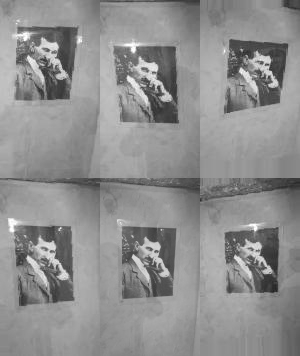
\includegraphics[scale=0.5]{./slike/augmented_dataset.jpeg}
        \end{center}
    \end{column}
    \end{columns}
\end{frame}
%-----------------------------------------------------------------
\begin{frame}{Trening mreže}
    \begin{itemize}
        \item Dobijen skup podataka od 18000 instanci rezolucije 100$\times$178
        \item Izvršen trening sa trening skupom od 12600 instanci (70\%  celog skupa)
        \item Korišćen algoritam optimizacije Adam \cite{adam}
        \item Izabrano 40 epoha, i serija veličine 32 (eng. batch)
        \item Trenirano na grafičkoj karti Nvidia GeForce 1060 GTX
        \item Trening trajao oko 1h
        \item Dobijena preciznost od 99.83\%
        \item Korišćene biblioteke \texttt{TensorFlow} \cite{tensorflow} i \texttt{keras} \cite{keras}
    \end{itemize}
\end{frame}
%-----------------------------------------------------------------
\begin{frame}{Arhitektura konvolutivne mreže}
    \begin{columns}
    \begin{column}{0.75\textwidth}
        \begin{itemize}
            \item \texttt{conv2d\_1} - veličina 3$\times$3, 32 filtera
            \item \texttt{conv2d\_2} - veličina 3$\times$3, 64 filtera
            \item \texttt{max\-pooling2d\_1} - agregacija veličine 2$\times$2
            \item \texttt{conv2d\_1} - kovolutivni sloj, veličina 3$\times$3
            \item \texttt{dropout\_1} - stepen 0.25 \cite{dropout}
            \item \texttt{flatten\_1} - serijalizuje vektor
            \item \texttt{dense\_1} - neuronska mreža sa 128 neurona 
            \item \texttt{dropout\_2} - stepen 0.25
            \item \texttt{dense\_2} - neuronska mreža sa 9 neurona i funkcijom softmax
        \end{itemize}
    \end{column}
    \begin{column}{0.25\textwidth}  %%<--- here
        \begin{center}
            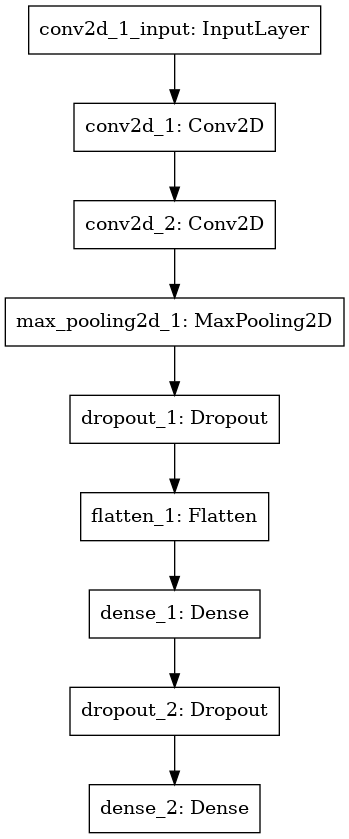
\includegraphics[scale=0.21]{./slike/model01.png}
        \end{center}
    \end{column}
    \end{columns}
\end{frame}
%-----------------------------------------------------------------
\section{Dalji rad}
%-----------------------------------------------------------------
\begin{frame}{Dalji rad}
    \begin{itemize}
        \item Sagledati kako se dobijeni model pokazuje u praksi nakon nekoliko meseci
        \item Analizirati pogrešno klasifikovane slike
        \item Probati nekoliko drugih arhitektura mreže
        \item Pokušati klasifikaciju slika koristeći druge metode mašinskog učenja
        \item Evaluirati opterećenje servera pri nekoliko istovremenih klasifikacija (i poboljšati)
        \item Povećati skup podataka
    \end{itemize}
\end{frame}

%\begin{columns}
%\begin{column}{0.3\textwidth}
    %\begin{center}
        %\includegraphics[scale=0.17]{./slike/interpolant_code2.png}
    %\end{center}
%\end{column}
%\begin{column}{0.7\textwidth}  %%<--- here
	%\begin{itemize}
    %\item Интерполанта је доказ да су скупови $A$ и  $B$ дисјунктни
    %\item Доказивач теорема рачуна вредности за променљиве $x$ и  $y$
    %\item Добија се скуп инстанци над којима се може тренирати модел машинског учења
    %\end{itemize}
%\end{column}
%\end{columns}

%\end{frame}

%-----------------------------------------------------------------
\begin{frame}
\Huge{\centerline{Pitanja?}}
\end{frame}
%-----------------------------------------------------------------
\begin{frame}
\Huge{\centerline{Hvala na pažnji!}}
\end{frame}
%-----------------------------------------------------------------

\begin{frame}[t, allowframebreaks]
\frametitle{Bibliografija}
\bibliographystyle{apalike}
\bibliography{seminarski}
\end{frame}


%-----------------------------------------------------------------
\end{document}
